%!TeX root =  ../../thesis.tex

\section{Klávesnice}
Pro dostatečné ovládání byla vybrána klávesnice s pěti tlačítky: Right, Left, Power, Auto, Menu. Tlačítko “Power” začne test kabelu, tlačítka “Left” a “Right” se používají k posouvání rotačního meny a tlačítko “Menu” přepíná mezi třemi zdrojovými konektory, nebo-li přepíná mezi submeny.

\begin{figure}[H]
	\centering
	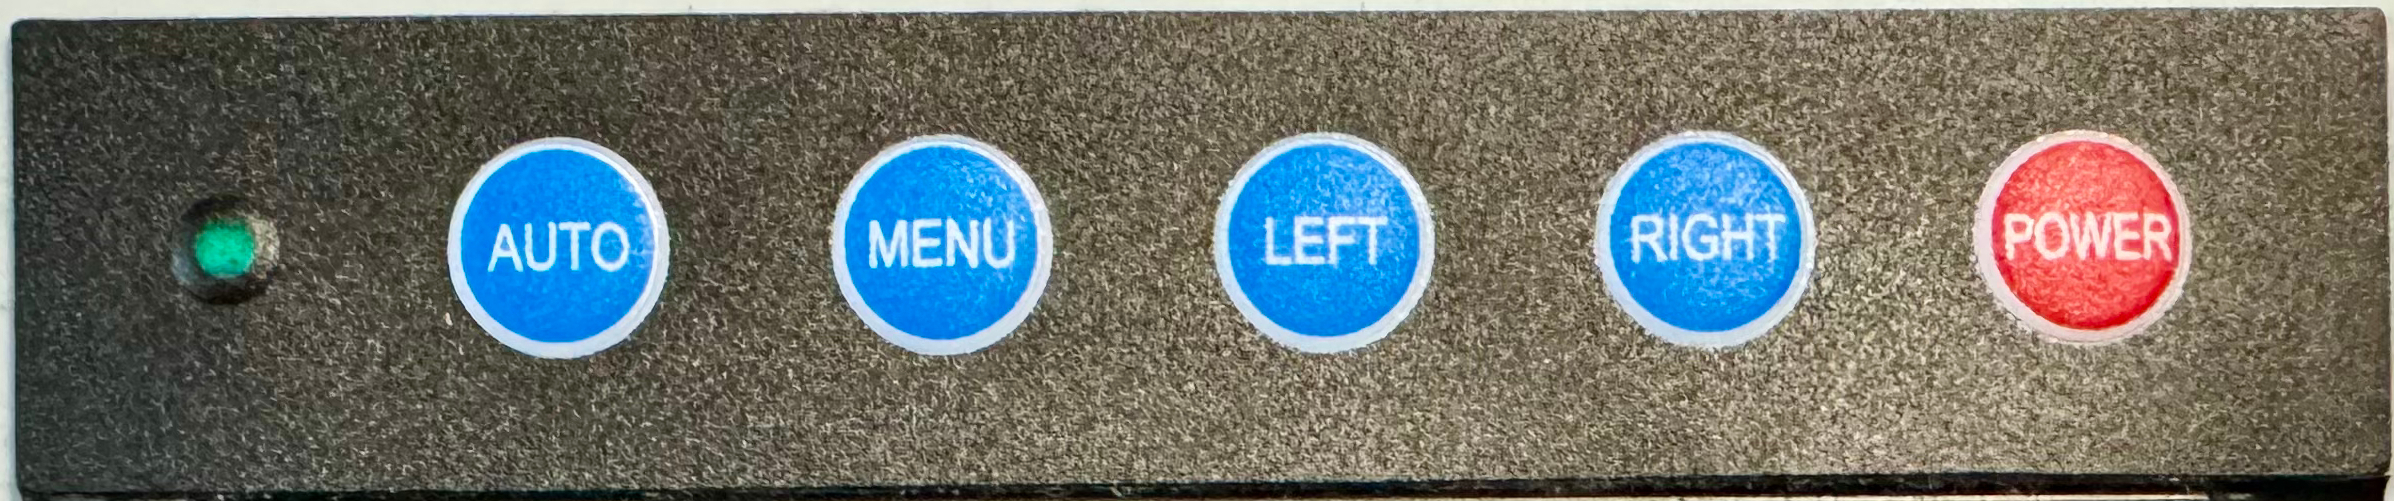
\includegraphics[width=0.9\textwidth]{pictures/keyboard.jpeg}
    	\caption{Klávesnice testeru}
   	\label{fig:keyborad}
\end{figure}

Na obrázku \ref{fig:keyborad} je vidět klávesnice/ovládací panel, kterým se tester ovládá.

\subsection*{Připojení k desce}
\begin{table} [h!]
	\caption{Pinové rozložení klávesnice}
	\label{table:pinKB}
	\centering
	\catcode`\-=12 % Because of czech
	\begin{tabular}[c]{|| c | c | c ||}
	\hline
		\multicolumn{3}{||c||}{Piny klávesničky} \\
	\hline
 		 \textbf{PIN} & \textbf{Tlačítko} & \textbf{Akce}\\
	\hline
		42 &  RIGHT & Posune rotační menu doprava\\
	\hline
		46 & POWER &  Začne testovat vybraný kabel\\
	\hline
		48 & LEFT & Posune rotační menu doleva\\
	\hline
		50 & MENU & Přepne menu na další zdrojový konektor \\
	\hline
		52 & AUTO & Začne testovat vybraný kabel\\
	\hline
	\end{tabular}
\end{table}

V tabulce  \ref{table:pinKB} je popsáno, které piny jsou napojeny na konkrétní tlačítko a co je akce vykonávaná při stisku tlačítka.
